\documentclass[10pt,a4paper]{article}

\usepackage[utf8]{inputenc}
\usepackage[T1]{fontenc}

%%%%%%%%%%% Own packages
\usepackage[a4paper, margin=1in]{geometry}
\usepackage{multicol}
\usepackage{lipsum}
\usepackage{natbib}

% Header/footer
\usepackage{fancyhdr}
\pagestyle{fancy}
\renewcommand{\headrulewidth}{0pt}

% Footnotes at bottom of page
\usepackage[bottom,marginal]{footmisc}
% \setlength{\footnotemargin}{1.8em}

% Maths
\usepackage{physics}
\usepackage{esdiff}
\usepackage{cancel}
\usepackage{amstext,amsbsy,amssymb,mathtools}
\usepackage{times} 
\usepackage{siunitx}
\usepackage{tensor}

%% Graphics
\usepackage{caption}
\captionsetup{margin=20pt,font=small,labelfont=bf}
%\renewcommand{\thesubfigure}{(\alph{subfigure})} % Style: 1(a), 1(b)
%\pagestyle{empty}
\usepackage{graphicx} % Include figure files

% Listsings and items
\usepackage[page]{appendix}
\usepackage[shortlabels]{enumitem}
\setenumerate{wide,labelwidth=!, labelindent=0pt}
\usepackage{varioref}
\usepackage{hyperref}
\usepackage{cleveref}

% Paragraph indent and skip
\setlength{\parindent}{2em}
\setlength{\parskip}{1em}
\setlength\extrarowheight{5pt}

%% User units
\DeclareSIUnit \parsec {pc}

%% User commands
\providecommand{\qwhere}
{%
\ensuremath{
,\quad \text{where} \quad%
}
}
\providecommand{\rCDM}
{\ensuremath{
\textrm{CDM}
}
}

\allowdisplaybreaks
\title{AST5220 Cosmology \rm{II}\\ 
\vspace{5mm}Milestone 3 - The Evolution of Structure in the Universe}
\author{Jakob Borg}
%%%%%%%
\begin{document}
%%%%%%%
\maketitle
\lhead{Milestone 3 AST5220}
\rhead{Jakobbor}
%%%%%%%%

\section{Introduction}
\label{sec:Introduction}
This report sums up milestone three of four in our way to compute the cosmic microwave background (CMB) power spectrum. In part one and two we've calculated the background evolution giving us the expansion history of the Universe\footnote{Milestone 1, \cite{milestone1}}, and it's ionization history giving us the optical depth and visibility function\footnote{Milestone 2, \cite{milestone2}}, all as functions of the logarithmic scale factor $x$.

Now in part three we are ready to calculate how the early small perturbations set up by inflation in the photon-baryon-dark-matter fluid of the early Universe evolves from shortly after inflation until today, also as functions of $x$. The perturbations are described by the Boltzmann equations for each component and the Einstein equations for the perturbations in the metric, see \cref{subsec:Theory/Coupled equations}. These perturbations will behave differently on different scales, dependent on the time they become causally connected to them self, see \cref{subsec:Method/Horizon entry}. To simplify our equations dramatically we will perform all calculations and subsequent analysis in Fourier space with wave number $k$. In Fourier space we can look at how different scales, characterized as $\lambda \propto 1/k$, evolve independently. The final goal of this milestone is therefore to compute two dimensional functions able to evaluate the following main physical quantities which will be discussed in \cref{sec:Results}
\begin{alignat*}{4}
  & \text{Gravitational potentials :} &\quad& \Psi(x,k) &\quad& \Phi(x,k) &
  \\
  & \text{Matter perturbations :}     &\quad& \delta_{\rCDM}(x,k) &\quad& v_{\rCDM}(x,k) &
  \\
  &                                  &\quad& \delta_{b}(x,k) &\quad& v_{b}(x,k) &
  \\
  & \text{\parbox{3cm}{Photon perturbations as multipoles} :}
                                  &\quad& \Theta_\ell(x,k) &\quad& \qfor* \ell = {0,1}&
\end{alignat*}%
where \rm{CDM} and $b$ is short for cold dark matter and baryons. See \cref{subsec:Theory/Coupled equations} for a short description of the photon multipoles following \cite{Calin} and \cite{Dodelson}.  Note that we are not including neutrinos or polarization in this model.

The full project can be found on GitHub, here are link to the \href{https://github.com/Lilleborg/AST5220-Cosmology2/tree/master/Numerical_projects}{projects main directory}\footnote{URL: \url{https://github.com/Lilleborg/AST5220-Cosmology2/tree/master/Numerical_projects}}. All computation and calculations are done in "C++", with the source code found \href{https://github.com/Lilleborg/AST5220-Cosmology2/tree/master/Numerical_projects/src}{here}\footnote{URL: \url{https://github.com/Lilleborg/AST5220-Cosmology2/tree/master/Numerical_projects/src}}. The main work for this milestone is concentrated into the \textit{Perturbations.h} class, building upon the work done in previous milestones. Note also that some of the code in the class is done in preparation for the next milestone, mainly computing the temperature source function, and this will not be discussed in detail here, but briefly mentioned in \cref{subsubsec:Method/Two ODE systems}.

%  _______ _                           
% |__   __| |                          
%    | |  | |__   ___  ___  _ __ _   _ 
%    | |  | '_ \ / _ \/ _ \| '__| | | |
%    | |  | | | |  __/ (_) | |  | |_| |
%    |_|  |_| |_|\___|\___/|_|   \__, |
%                                __/ |
%                               |___/ 
\section{Theoretical Background}
\label{sec:Theory}

\subsection{The Coupled System of Equations}
\label{subsec:Theory/Coupled equations}

With the background cosmology of the Universe solved in \cite{milestone1} we can now focus on the perturbations alone, and simply add them to the background solutions to describe the full Universe with Einsteins field equations. When we measure the temperature of the CMB we actually measure this deviation from the background solution set up by the perturbations. The following equations for the different components are thus describing the perturbations of the corresponding quantities obtained from the Boltzmann equation for photons, \rCDM and baryons.

Following \cite{Calin} we describe a perturbed universe with the Newtonian gauge, writing the perturbed metric as 
\begin{equation}
\tensor{g}{_\mu_\nu} =
  \begin{pmatrix}
    -(1+2\Psi) & 0
    \\
    0 & a^2\delta_{ij}(1+2\Phi)
  \end{pmatrix}
\end{equation}
where $\Phi$ and $\Psi$ are interpreted as small gravitational potentials set up by the perturbations. Using this metric we obtain equations for the potentials using Einsteins equation.

Using the logarithmic scale factor $x$ as time variable we can write the resulting coupled equations from Einsteins equation and the Boltzmann equations as follows, where $^\prime$ denotes derivatives with respect to $x = \ln(a)$:
\begin{itemize}
\item Potential or metric perturbations
\begin{align}
  \Psi &= -\Phi - \frac{12H_0^2}{c^2k^2a^2}\Omega_{r0}\Theta_2 \label{eq:Psi}
  \\
  \Phi^\prime &= \Psi - \frac{c^2k^2}{3\mathcal{H}^2} \Phi + \frac{H_0^2}{2\mathcal{H}^2}
  \left[\Omega_{\rm CDM 0} a^{-1} \delta_{\rm CDM} + \Omega_{b0} a^{-1} \delta_b + 4\Omega_{r0}
  a^{-2}\Theta_0\right]
\end{align}%
Note that written on this form we don't have an equation of motion for $\Psi$, but instead express it in terms of the other dynamical perturbations $\Phi$ and $\Theta_2$.

\item The matter perturbations
\begin{align}
  \delta_{\rm CDM}^\prime &= \frac{ck}{\mathcal{H}} v_{\rm CDM} - 3\Phi^\prime \\
  v_{\rm CDM}^\prime &= -v_{\rm CDM} -\frac{ck}{\mathcal{H}} \Psi \\
  \delta_b^\prime &= \frac{ck}{\mathcal{H}}v_b -3\Phi^\prime \\
  v_b^\prime &= -v_b - \frac{ck}{\mathcal{H}}\Psi + \tau^\prime R(3\Theta_1 + v_b)
\end{align}
where
\begin{equation}
  R = \frac{4\Omega_{r0}}{3\Omega_{b0}a}.
  \label{eq:R}
\end{equation}

\item The photon temperature perturbations
\begin{align}
  \Theta^\prime_0 &= -\frac{ck}{\mathcal{H}} \Theta_1 - \Phi^\prime,
  \\
  \Theta^\prime_1 &=  \frac{ck}{3\mathcal{H}} \Theta_0 - \frac{2ck}{3\mathcal{H}}\Theta_2 +
  \frac{ck}{3\mathcal{H}}\Psi + \tau^\prime\left[\Theta_1 + \frac{1}{3}v_b\right],
  \label{eq:dipole ODE}
  \\
  \Theta^\prime_\ell &= \frac{\ell ck}{(2\ell+1)\mathcal{H}}\Theta_{\ell-1} - \frac{(\ell+1)ck}{(2\ell+1)\mathcal{H}}
  \Theta_{\ell+1} + \tau^\prime\left[\Theta_\ell - \frac{1}{10}\Pi
  \delta_{\ell,2}\right], \quad\quad 2 \leq \ell < \ell_{\textrm{max}}
  \\
  \Theta_{\ell}^\prime &= \frac{ck}{\mathcal{H}}
  \Theta_{\ell-1}-c\frac{\ell+1}{\mathcal{H}\eta(x)}\Theta_\ell+\tau^\prime\Theta_\ell,
  \quad\quad \ell = \ell_{\textrm{max}}
\end{align}
where $\Pi$ is a sum over the quadrupole perturbation $\Theta_2$ and perturbations of the photon polarization, but we exclude polarization from our model and thus define $\Pi \equiv \Theta_2$. The photon perturbations are here directly presented in the expanded form using Legendre polynomials.

Note that the multipoles in reality sets up an infinite hierarchy of equations, where $\ell_{\rm{max}} \rightarrow \infty$, but we have to define a maximum number of equations and thus have a separate equation for $\Theta_{\ell_{\rm{max}}}$. To balance the accuracy of this abrupt stop in the hierarchy with the required computation time we define $\ell_{\rm{max}}=8$, made possible by a neat trick called line of sight integration which will be used in the next milestone when we actually need all the higher order multipoles up to $\ell \sim 1200$. For this milestone, as mentioned in \cref{sec:Introduction}, we will only focus on the quantities we have a physical intuitive description of, namely the monopole and dipole, but we include up to $9$ multipoles to reduce the error caused by not using the full infinite expansion.

% , where the full photon perturbation is
% \begin{equation}
%   \Theta = 
% \end{equation}
\end{itemize}

\subsubsection{Tight Coupling Regime}
\label{subsubsec:Theory/Tight Coupling}
In the early universe we know from \cite{milestone2} that the optical depth is very large, so the mean free path of photons is very short. This means that electrons in the early Universe only is affected by photons, or in other words temperature fluctuations, that are in the close vicinity. Thus the photons and electrons are tightly coupled and behave like a electron-photon fluid. During this period of tight coupling we will only have very smooth fluctuations since the small fluctuations, and hence gradients, are efficiently washed out due to system being in thermal equilibrium. Therefor the only relevant quantities affecting the baryon-photon fluid are
\begin{enumerate}
  \item the mean temperature, quantified by the monopole $\Theta_0$,
  \item the dipole itself,  $\Theta_1$, given by the velocity of the electron-photon fluid due to the Doppler effect
  \item and the quadrupole, $\Theta_2$, which is the only relevant source of polarization in this early regime
\end{enumerate}
and the higher order multipoles are negligible. Thus at early times we don't need to include higher order multipoles than $\ell = 0$ and $1$ in our coupled system of differential equations. For the higher order multipoles we will simply use a set of algebraic equations as given by the initial conditions which will be described next in \cref{subsubsec:Theory/Initial conditions}.

We also have a numerical issue in the early times, lurking in \cref{eq:dipole ODE}. Early on the perturbations are really small, with small velocities, and thus the sum in $\left[\Theta_1 + \frac{1}{3}v_b\right]$ is very small. This is multiplied by the derivative of the optical depth $\tau^\prime$, which is in turn very large following the order of magnitude of the optical depth it self. The result is a very unstable numerical system, where the tiniest error in the mentioned sum will lead to a large error in the system of differential equations. To solve this we use a clever approximation for $\left[3\Theta_1 + v_b\right]$ following \cite{Calin}, resulting in the following equations for $\Theta_1$ and $v_b$
\begin{align}
  q &= \frac{-[(1-R)\tau^\prime + (1+R)\tau^{\prime\prime}](3\Theta_1+v_b) -
  \frac{ck}{\mathcal{H}}\Psi + (1-\frac{\mathcal{H}^\prime}{\mathcal{H}})\frac{ck}{\mathcal{H}}(-\Theta_0 +
  2\Theta_2) - \frac{ck}{\mathcal{H}}\Theta_0^\prime}{(1+R)\tau^\prime + \frac{\mathcal{H}^\prime}{\mathcal{H}} -
  1}
  \\
  v_b^\prime &= \frac{1}{1+R} \left[-v_b - \frac{ck}{\mathcal{H}}\Psi + R(q +
  \frac{ck}{\mathcal{H}}(-\Theta_0 + 2\Theta_2) - \frac{ck}{\mathcal{H}}\Psi)\right]
  \\
  \Theta^\prime_1 &= \frac{1}{3} (q - v_b^\prime)
\end{align}
where again $R$ is from \cref{eq:R}.

\subsubsection{Initial Conditions}
\label{subsubsec:Theory/Initial conditions}
As mentioned when presenting the system of equations, $\Psi$ in \cref{eq:Psi} is not a dynamical quantity in the system. Since the system is linear we are free to choose any normalization of $\Psi$ as we want when we solve the system, and just rescale the quantities later appropriately. For now we simply choose to set the initial condition for $\Psi = -\frac{2}{3}$ in \cref{eq:Psi init}, and we will come back to this is the next milestone when we compute the CMB and matter power spectra. It can be shown that the rest of the initial conditions follows from this, assuming adiabatic initial conditions set up by an adiabatic inflation period.
\begin{align}
  \Psi &= -\frac{2}{3} \label{eq:Psi init}
  \\
  \Phi &= -\Psi
  \\
  \delta_{\rm CDM} &= \delta_b = -\frac{3}{2} \Psi 
  \\
  v_{\rm CDM} &= v_b = -\frac{ck}{2\mathcal{H}} \Psi
  \\
  \Theta_0 &= -\frac{1}{2} \Psi 
  \\
  \Theta_1 &= \frac{ck}{6\mathcal{H}}\Psi 
  \\
  \Theta_2 &= -\frac{20ck}{45\mathcal{H}\tau^\prime} \Theta_1,
  \\
  \Theta_\ell &= -\frac{\ell}{2\ell+1} \frac{ck}{\mathcal{H}\tau^\prime} \Theta_{\ell-1} \quad \qfor \ell > 2
\end{align}

%  __  __      _   _               _ 
% |  \/  |    | | | |             | |
% | \  / | ___| |_| |__   ___   __| |
% | |\/| |/ _ \ __| '_ \ / _ \ / _` |
% | |  | |  __/ |_| | | | (_) | (_| |
% |_|  |_|\___|\__|_| |_|\___/ \__,_|
\section{Method}
\label{sec:Method}

\subsection{Creating Two Dimensional Functions}
\label{subsec:Method/2D functions}
For the integration we are doing in the final milestone, to compute the CMB power spectrum, we need solutions to our equations in Fourier space and time, expressed in terms of the wave number $k$ and the logarithmic scale factor $x$. Therefore our goal here is to create two-dimensional splines of the main physical quantities mentioned in \cref{sec:Introduction}. Note that we also create a few splines related to the calculations for the next milestone, which will not be discussed here.

In order to do so we solve the systems of equations presented in \cref{subsec:Theory/Coupled equations} in two ranges of $k$-values and $x$-values, with $2000$ $x$-values linearly spaced between $x_{\rm{min}} = -15$ to $x_{\rm{max}}=0$, and $150$ $k$s logarithmically spaced between $k_{\rm{min}} = \SI{5e-5}{\per\mega\parsec}$ to $k_{\rm{max}} = \SI{0.3}{\per\mega\parsec}$. All the different wave numbers are independent, so we simply loop over the range of $k$s solving the ODE-system in a similar fashion as in the previous milestones, taking into consideration the two regimes presented in \cref{subsec:Theory/Coupled equations}.

\subsection{Solving in Two Regimes}
\label{subsec:Method/Solving in two regimes}

\subsubsection{Determining the Tight Coupling Regime}
\label{subsubsec:Method/Determine TC}
The first thing we need for each value of $k$ is to find the transition between the tight coupling regime and the full system. For this we follow the convention presented by \cite{Calin} and define the tight couple regime to end when $\abs*{\tau^\prime(x)}<10$ or $\abs*{\tau^\prime(x)}<10\frac{ck}{\mathcal{H}}$, and no later than at start of recombination which we define as when the free electron fraction $X_e(x) < 0.99$. The value and index of this transition, $x_{\textrm{tc end}}$, is used to create two sets of ranges in $x$, and we treat the systems appropriately in the two regimes.

\subsubsection{Two Sets of Coupled Equations}
\label{subsubsec:Method/Two ODE systems}
We create one system of coupled ODE-equations for the tight coupled regime, and one for the full system including the higher order multipoles, and solve them using the Runge-Kutta 4 ODE-solver from the GSL library. When setting up these systems in our numerical methods for each regime we have to carefully implement them in the right order presented in \cref{subsec:Theory/Coupled equations}.

When extracting the solutions from the ODE-solvers and storing the result we update the non-dynamical quantities that are not treated by the ODE-solver following the algebraic equations. The solutions in each regime are stored into the same two-dimensional arrays in $k$ and $x$, which is splined in the end giving us the two-dimensional callable methods, or functions, we want.

\subsubsection{Setting Initial Condtions}
\label{subsubsec:Method/setting initial conditions}
To set the initial conditions we create two methods, again one for each regime. For the tight coupling we regime we initialize with the equations presented in \cref{subsubsec:Theory/Initial conditions} up to $\ell = 2$. For the full regime after $x_{\textrm{tc end}}$ we use the solutions at the end of the tight coupled regime to initialize the quantities at time $x_{\textrm{tc end}}$. Here we also have to initialize the higher order multipoles of $\ell > 2$ following \cref{subsubsec:Theory/Initial conditions}.

\subsection{Horizon Entry}
\label{subsec:Method/Horizon entry}
To help analyze our results we find the point in time where the perturbations of the different scales $k$ enter inside the particle horizon and become causally connecter. The perturbations are considered well out of the horizon when $k\eta(x) \ll 1$, and we define the point of entry when
\begin{equation}
  \eta(x_{\rm{Horizon,k}}) = \frac{1}{k}
  \label{eq:Horizon entry}
\end{equation}
where $\eta(x)$ is the conformal time from \cite{milestone1}.

%  _____                 _ _       
% |  __ \               | | |      
% | |__) |___  ___ _   _| | |_ ___ 
% |  _  // _ \/ __| | | | | __/ __|
% | | \ \  __/\__ \ |_| | | |_\__ \
% |_|  \_\___||___/\__,_|_|\__|___/
\section{Results}
\label{sec:Results}
As in the previous milestones there are a few things in common with all the figures displaying the results. The background is colored to show the three different background regimes, blue being the radiation dominated regime, red the matter dominated, and green the current day regime dominated by dark energy, as described in \cite{milestone1}. 

The yellow area indicates the regime of recombination, but this time defined when the visibility function is effectively non-zero, and not when the free electron fraction starts to decay. The reason for this will be more evident in the next milestone when we compute the source function used in the power spectrum calculations, being heavily dependent on the visibility function. We find the starting time of this period using the results from \cite{milestone2}, when $X_e(x_{\rm{rec}}) = 0.5$, and the end time when $\tilde{g}(x_{\textrm{rec end}}) < 0.1$ after its peak at $\tau(x_\star) =1$.

For all the main physical quantities we present six different scales, or wave numbers. The values are selected in order to display two solutions from each type of scale-regime;
\begin{itemize}
  \item large scales, or super-horizon scales, with small wave numbers $k=\{0.001,\,0.0005\}\,\si{\per\mega\parsec}$ shown in pink and orange
  \item intermediate scales, entering right before and after radiation-matter-equality, shown in purple and green  with numbers $k=\{0.013,\,0.007\}\,\si{\per\mega\parsec}$
  \item small scales, entering early in the radiation dominated regime, shown in blue and red  with large wave numbers $k=\{0.3,\,0.1\}\,\si{\per\mega\parsec}$.
\end{itemize}
For each scale we mark the time of horizon entry following \cref{eq:Horizon entry} in a vertical dotted line in the corresponding colors. In the following discussion the different scales are also referred to by their color for simplicity.

In the presented plots we also show the solutions in times beyond todays value of $x$, until $x=2$. These results are mainly to help visualize what happens in a Universe dominated by dark energy, and must not be taken to seriously as we have defined the optical depth to be zero at $x=0$, and is not accurate for times $x>0$.

The full calculation for the entire grid, for $150$ $k$-values and $2000$ $x$-values, are done in $\sim \SI{6.7}{s}$.

\subsection{Matter Perturbations}
\label{subsec:Results/Matter pert}
The perturbations for \rCDM and baryons are presented in \cref{fig:matter pert}. Here we have to mention that these quantities are not gauge-invariant, and the solutions could therefore follow other proportionalities to time in different gauges.

First interpreting the pressure-less \rCDM which is able to start growing in the radiation dominated regime, we see that the perturbations on all scales remain constant until they enter the horizon and becomes causally connected, so that gravity can start contracting them. The velocities of the perturbations increase from close to zero until horizon entry, consistent with the horizon being bigger and bigger and thus the part of the causally connected mass within increasing, pulling more and more, so that the matter falls gradually faster and faster. When the perturbation enters the horizon it is considered a growing mode, growing differently depending on which time regime it entered.

Perturbations on scales entering in the radiation dominated regime, like the blue and red, will first start to grow in what looks like an exponential growth, before it is affected by Meszaros suppression and grows like $\delta_{\rCDM} \propto \ln(a) = x$. At this point the velocities are also suppressed, consistent with the mode growing slower due to the suppression. When we go beyond the radiation-matter-equality the Meszaros suppression stops and the growing modes follow $\delta_{\rCDM} \propto a = e^x$. Here again the velocities start to increase as the matter in the perturbations are pulled faster and faster into the gravitational potential wells.

Perturbations on scales entering around or after this equality, like the purple and green, are not affected by the Meszaros suppression, and we see the perturbations starting to grow directly into the $\delta_{\rCDM} \propto a$ relationship, with the velocities not being suppressed at all. We note that the velocities for all the different scales are shifted in value relative to each other so that they all are about $v \sim 0.3$ at horizon entry. The perturbations continue to grow like this until the current regime dominated by dark energy and expansion. The accelerated expansion will cause all the perturbations to stop growing, remaining constant $\delta_{\rCDM} \sim \textrm{constant}$, with decreasing velocities.

\begin{figure}[ht!]
  \centering
  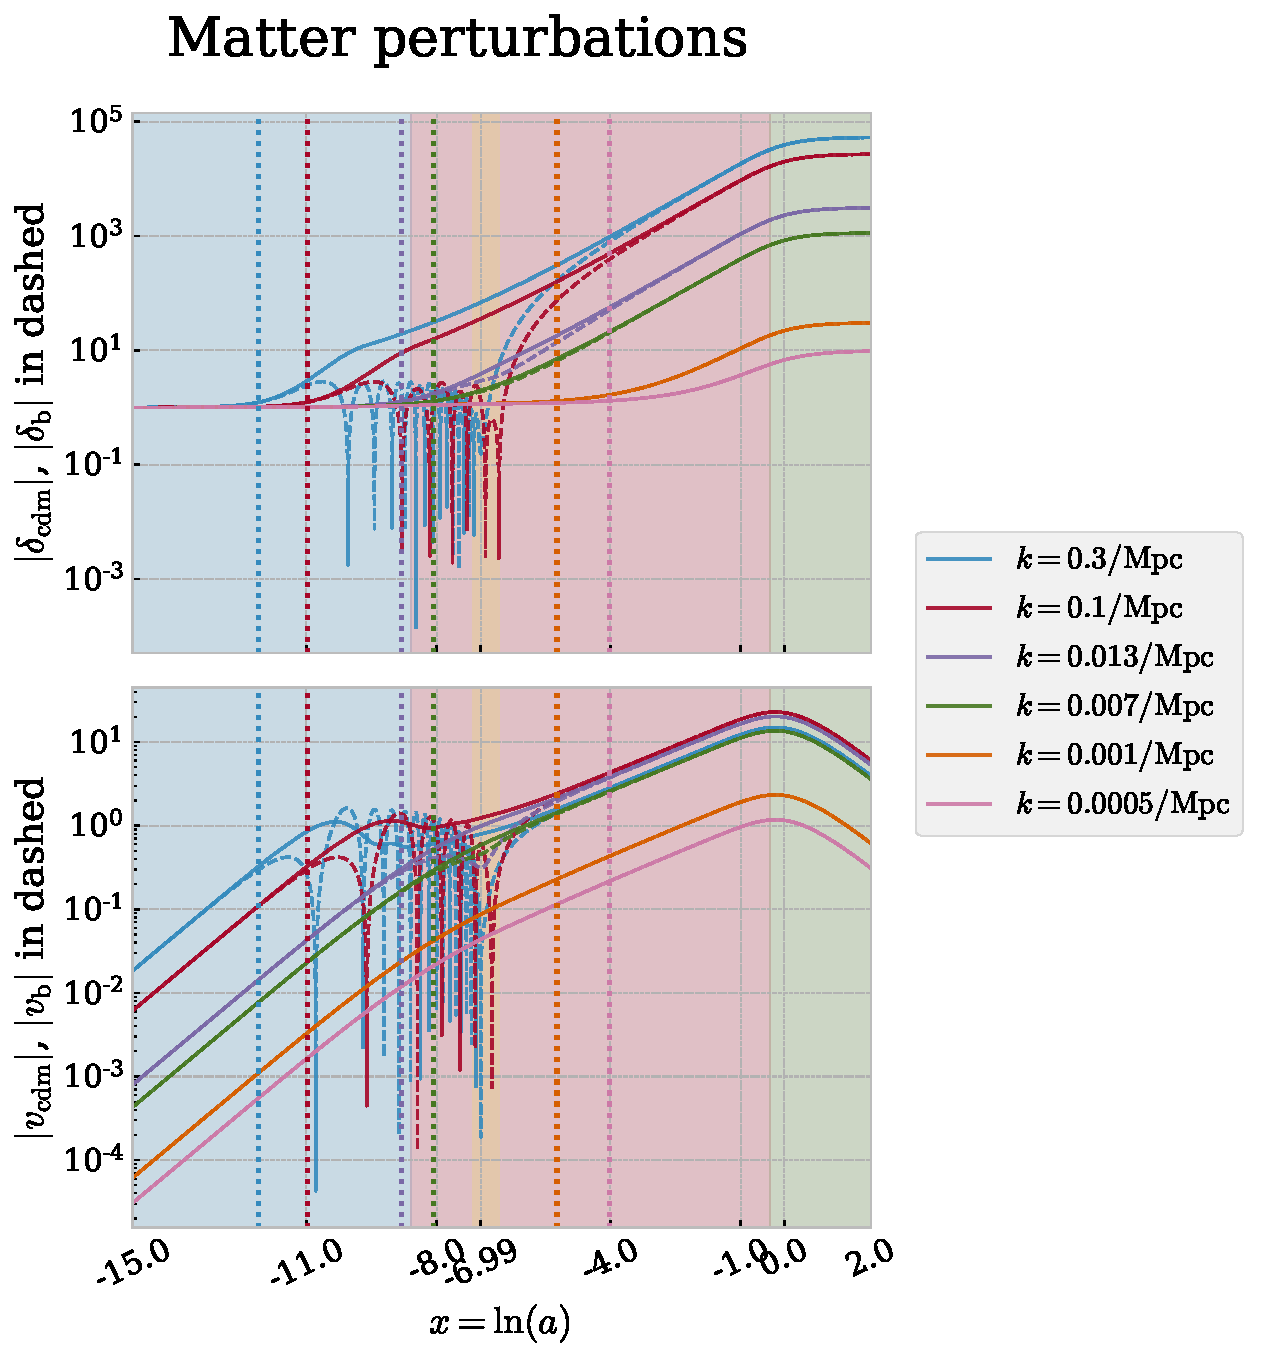
\includegraphics[scale=0.5]{../figs/matter_pert.pdf}
  \caption{Matter perturbations, \rCDM shown in solid lines, baryons in dashed, for the six different scales $k$. The top panel shows the density contrast $\delta$ and the lower panel shows the absolute value of the velocity $v$, both in Fourier space.}
  \label{fig:matter pert}
\end{figure}

Now looking at the baryonic perturbations we see much of the same behavior, with the only exception being scales entering the horizon before the end of recombination not growing beyond a certain value, but instead oscillating. This is due to their tight coupling with the photons and the early baryon-photon fluid. This will be evident in \cref{fig:Photon pert} as well when we look at the photon perturbations. The equations for the perturbations can be expressed on the form of a driven harmonic oscillator, with gravity being the attracting force and radiation pressure the repulsive force. This balance will cause the baryonic perturbations entering before the decoupling of the baryons and photons to oscillate, first being compressed when the gravitational force is dominating before the radiation pressure starts to dominate and the perturbation is rarified. The large scale perturbations, entering after recombination is not affected by this coupled state, and will not oscillate but just follow the dark matter perturbations.

This effect is clearly visible on the scales of the red and blue perturbation, oscillating heavily until the end of recombination. At this point the baryons are not coupled to the photons any more, and are free to fall into and follow the large gravitational potential wells set up by the dark matter perturbations. On the purple and green scales we can see a minor effect of this radiation pressure, causing a slight delay on the baryons growth relative to the \rCDM, before catching up again. This effect is a bit more evident on the purple scale entering just before the radiation-matter-equality, than the green entering right after the equality, consistent with the purple one being slightly more affected by radiation. The velocities follow the oscillations, but with a phase shift of $\frac{\pi}{2}$ so that the minimum value of the velocity corresponds to the maximum size of the perturbation, and vise versa, consistent with the harmonic oscillator description. For both the densities and the velocities we see how the early oscillations are dampened over time closer to recombination, due to diffusion dampening caused by the mean free path of the photons increasing with the decreasing optical depth.

\subsection{Photon perturbations}
\label{subsec:Results/Photon pert}
In \cref{fig:Photon pert} the monopole and dipole of the photon perturbations are shown, with some scaling so we can interpret the quantities as the perturbation's density\footnote{Or in other words temperature.} and velocity. Again we see much of the same behavior as for the baryon perturbations before recombination, due to their tight coupling. The perturbations are constant before entering the horizon. The small scales in red and blue that enters early starts oscillating heavily together with the baryons, with the oscillations being dampened onward in time until decoupling after recombination. Again we see that the velocities are following the density in a similar fashion as for the baryons, being phase shifted by $\frac{\pi}{2}$.

\begin{figure}[ht!]
  \centering
  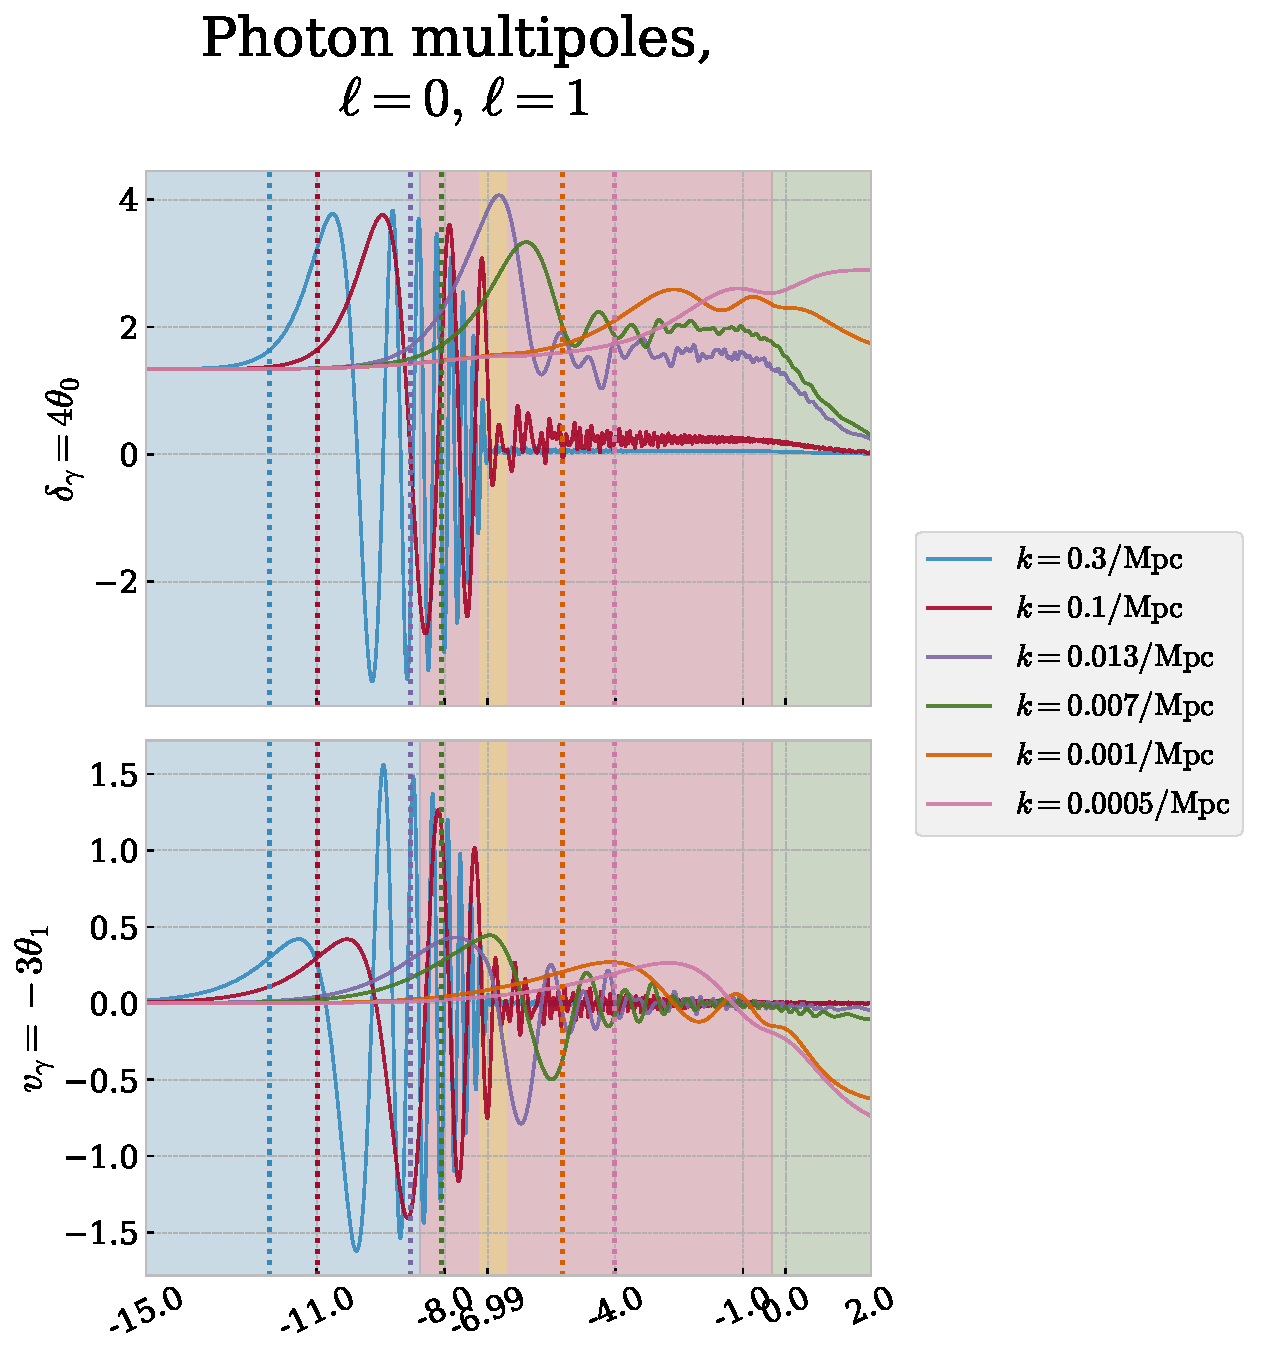
\includegraphics[scale=0.5]{../figs/multipole_pert.pdf}
  \caption{The monopole and dipole of the photon perturbations, here shown interpreted as the photon density contrast displayed in the top panel and a the velocity of the perturbation in the lower panel, both in Fourier space.}
  \label{fig:Photon pert}
\end{figure}

After decoupling, the optical depth has dropped significantly, and the photons are free to move more or less unhindered and no longer collapses together with the baryons. The dampening of the harmonic oscillations cause the perturbations to eventually be more or less constant, until the dark energy dominated regime when expansion causes them to start decay to zero.

The purple and green scales are barely affected by the coupled oscillated regime, and undergoes only a single peak before decoupling, while the orange and pink scales enter well into the matter dominated regime and is not affected by the coupling.

\subsection{Gravitational potentials}
\label{subsec:Results/Grav potentials}
Last we present the gravitational potentials in \cref{fig:Gravitational potentials}. Here it is evident that $\Psi \approx -\Phi$, and thus we will keep to discussing $\Phi$ alone where it is inferred that $\Psi$ behaves similarly. Again are all scales constant before entering the horizon, and behaves quite differently depending on the time of entry. In our understanding of these gravitational potentials we think of them as a type of newtonian potential. On scales, like the blue and red, entering the horizon and being causally connected in the radiation dominated regime, the potentials are dominated by radiation energy which does not cluster efficiently. Thus the potentials decay rapidly when the monopole increases, but start to oscillate due to the baryon-photon-fluid oscillations until after decoupling.

When we enter into the matter dominated regime, the dominating energy contributor to the potentials are baryons and the \rCDM, which do indeed cluster and causes the potentials to be constant with growing matter perturbations. The larger scales have less time to collapse, like we see in the difference between the red and blue scale, and thus holds a larger constant value through the matter dominated regime. For the purple and green scales we see the slight effect of the one oscillation of the monopole before the matter perturbations are too dominating, resulting in minor a drop off from the initial value flattening out after recombination. The largest scales entering well inside the matter dominated regime are nearly unaffected from their initial conditions, and it can be shown to drop of by a factor of $9/10$ into the matter dominated regime, which is consistent with the way our solutions for the orange and pink scales behaves. Note that the potentials all starts to decay into the dark energy regime, where expansion causes even the largest potentials to be smoothed out.

\begin{figure}[ht!]
  \centering
  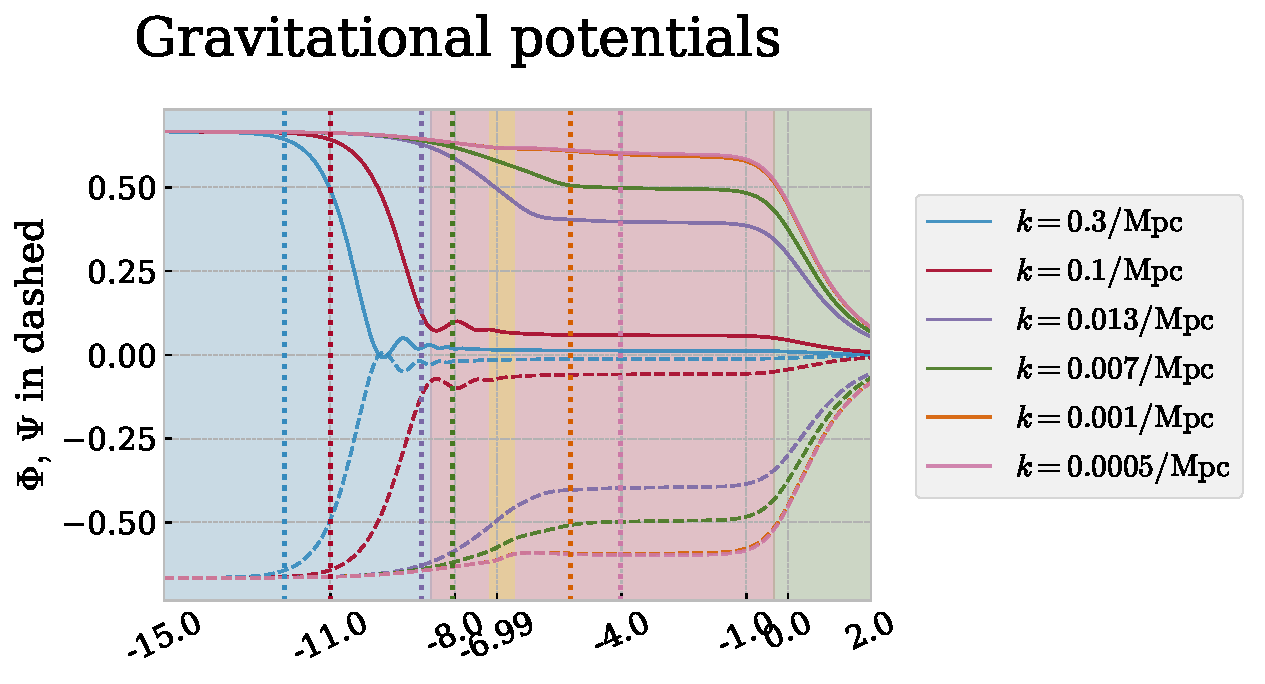
\includegraphics[scale=0.5]{../figs/potential_pert.pdf}
  \caption{Gravitational potentials, $\Phi$ shown in solid and $\Psi$ shown in dashed lines in Fourier space.}
  \label{fig:Gravitational potentials}
\end{figure}


%\pagebreak
\bibliographystyle{plainnat}
\bibliography{ref_milestone3}

\end{document}